%%%%%%%%%%%%%%%%%%%%%%%%%%%%%%%%%%%%%%%%%
% Beamer Presentation
% LaTeX Template
% Version 2.0 (March 8, 2022)
%
% This template originates from:
% https://www.LaTeXTemplates.com
%
% Author:
% Vel (vel@latextemplates.com)
%
% License:
% CC BY-NC-SA 4.0 (https://creativecommons.org/licenses/by-nc-sa/4.0/)
%
%%%%%%%%%%%%%%%%%%%%%%%%%%%%%%%%%%%%%%%%%




%----------------------------------------------------------------------------------------
%	PACKAGES AND OTHER DOCUMENT CONFIGURATIONS
%----------------------------------------------------------------------------------------

\documentclass[
	11pt, % Set the default font size, options include: 8pt, 9pt, 10pt, 11pt, 12pt, 14pt, 17pt, 20pt
	%t, % Uncomment to vertically align all slide content to the top of the slide, rather than the default centered
	aspectratio=169, % Uncomment to set the aspect ratio to a 16:9 ratio which matches the aspect ratio of 1080p and 4K screens and projectors
]{beamer}

\graphicspath{{Images/}{./}} % Specifies where to look for included images (trailing slash required)

\usepackage{booktabs} % Allows the use of \toprule, \midrule and \bottomrule for better rules in tables
\usepackage{tikz} % Allows the drawing of tikz
\usetikzlibrary{shapes,arrows,positioning,calc,backgrounds} % Tikz libraries required for the drawing of arrows, etc

%----------------------------------------------------------------------------------------
%	SELECT LAYOUT THEME
%----------------------------------------------------------------------------------------

% Beamer comes with a number of default layout themes which change the colors and layouts of slides. Below is a list of all themes available, uncomment each in turn to see what they look like.

%\usetheme{default}
%\usetheme{AnnArbor}
%\usetheme{Antibes}
%\usetheme{Bergen}
%\usetheme{Berkeley}
%\usetheme{Berlin}
%\usetheme{Boadilla}
%\usetheme{CambridgeUS}
%\usetheme{Copenhagen}
%\usetheme{Darmstadt}
%\usetheme{Dresden}
%\usetheme{Frankfurt}
%\usetheme{Goettingen}
%\usetheme{Hannover}
%\usetheme{Ilmenau}
%\usetheme{JuanLesPins}
%\usetheme{Luebeck}
\usetheme{Madrid}
%\usetheme{Malmoe}
%\usetheme{Marburg}
%\usetheme{Montpellier}
%\usetheme{PaloAlto}
%\usetheme{Pittsburgh}
%\usetheme{Rochester}
%\usetheme{Singapore}
%\usetheme{Szeged}
%\usetheme{Warsaw}

%----------------------------------------------------------------------------------------
%	SELECT COLOR THEME
%----------------------------------------------------------------------------------------

% Beamer comes with a number of color themes that can be applied to any layout theme to change its colors. Uncomment each of these in turn to see how they change the colors of your selected layout theme.

%\usecolortheme{albatross}
%\usecolortheme{beaver}
%\usecolortheme{beetle}
%\usecolortheme{crane}
%\usecolortheme{dolphin}
%\usecolortheme{dove}
%\usecolortheme{fly}
%\usecolortheme{lily}
%\usecolortheme{monarca}
%\usecolortheme{seagull}
%\usecolortheme{seahorse}
%\usecolortheme{spruce}
%\usecolortheme{whale}
%\usecolortheme{wolverine}

%----------------------------------------------------------------------------------------
%	SELECT FONT THEME & FONTS
%----------------------------------------------------------------------------------------

% Beamer comes with several font themes to easily change the fonts used in various parts of the presentation. Review the comments beside each one to decide if you would like to use it. Note that additional options can be specified for several of these font themes, consult the beamer documentation for more information.

\usefonttheme{default} % Typeset using the default sans serif font
%\usefonttheme{serif} % Typeset using the default serif font (make sure a sans font isn't being set as the default font if you use this option!)
%\usefonttheme{structurebold} % Typeset important structure text (titles, headlines, footlines, sidebar, etc) in bold
%\usefonttheme{structureitalicserif} % Typeset important structure text (titles, headlines, footlines, sidebar, etc) in italic serif
%\usefonttheme{structuresmallcapsserif} % Typeset important structure text (titles, headlines, footlines, sidebar, etc) in small caps serif

%------------------------------------------------

%\usepackage{mathptmx} % Use the Times font for serif text
\usepackage{palatino} % Use the Palatino font for serif text

%\usepackage{helvet} % Use the Helvetica font for sans serif text
\usepackage[default]{opensans} % Use the Open Sans font for sans serif text
%\usepackage[default]{FiraSans} % Use the Fira Sans font for sans serif text
%\usepackage[default]{lato} % Use the Lato font for sans serif text

%----------------------------------------------------------------------------------------
%	SUPRESSING AUX FILE DIRECTORY
%----------------------------------------------------------------------------------------

%----------------------------------------------------------------------------------------
%	SELECT INNER THEME
%----------------------------------------------------------------------------------------

% Inner themes change the styling of internal slide elements, for example: bullet points, blocks, bibliography entries, title pages, theorems, etc. Uncomment each theme in turn to see what changes it makes to your presentation.

%\useinnertheme{default}
\useinnertheme{circles}
%\useinnertheme{rectangles}
%\useinnertheme{rounded}
%\useinnertheme{inmargin}

%----------------------------------------------------------------------------------------
%	SELECT OUTER THEME
%----------------------------------------------------------------------------------------

% Outer themes change the overall layout of slides, such as: header and footer lines, sidebars and slide titles. Uncomment each theme in turn to see what changes it makes to your presentation.

%\useoutertheme{default}
%\useoutertheme{infolines}
%\useoutertheme{miniframes}
%\useoutertheme{smoothbars}
%\useoutertheme{sidebar}
%\useoutertheme{split}
%\useoutertheme{shadow}
%\useoutertheme{tree}
%\useoutertheme{smoothtree}

%\setbeamertemplate{footline} % Uncomment this line to remove the footer line in all slides
%\setbeamertemplate{footline}[page number] % Uncomment this line to replace the footer line in all slides with a simple slide count

%\setbeamertemplate{navigation symbols}{} % Uncomment this line to remove the navigation symbols from the bottom of all slides

%----------------------------------------------------------------------------------------
%	Roadmap
%----------------------------------------------------------------------------------------


\setbeamerfont{myTOC}{series=\bfseries, size=\Large}
\AtBeginSection[]{
        \frame{
            \frametitle{Roadmap}
            \tableofcontents[current]   
        }
    }

%----------------------------------------------------------------------------------------
%	Configuration of Footer
%----------------------------------------------------------------------------------------

\setbeamertemplate{navigation symbols}{} 

\makeatletter


\setbeamertemplate{footline}{%
  \raisebox{5pt}{\makebox[\paperwidth]{\hfill\makebox[10pt]{\scriptsize\insertframenumber}}}}

%----------------------------------------------------------------------------------------
%	PRESENTATION INFORMATION
%----------------------------------------------------------------------------------------

\title{Banking, Liquidity, and Bank Runs in an Infinite Horizon Economy} % The short title in the optional parameter appears at the bottom of every slide, the full title in the main parameter is only on the title page

\subtitle{By Mark Gertler and Nobuhiro Kiyotaki} % Presentation subtitle, remove this command if a subtitle isn't required

\author[Williams]{Nathan Williams} % Presenter name(s), the optional parameter can contain a shortened version to appear on the bottom of every slide, while the main parameter will appear on the title slide

\institute[Emory]{Emory University \\ \smallskip \textit{nathan.williams@emory.edu}} % Your institution, the optional parameter can be used for the institution shorthand and will appear on the bottom of every slide after author names, while the required parameter is used on the title slide and can include your email address or additional information on separate lines

\date[\today]{Macro Reading Group \\ \today} % Presentation date or conference/meeting name, the optional parameter can contain a shortened version to appear on the bottom of every slide, while the required parameter value is output to the title slide

%----------------------------------------------------------------------------------------
%	DOCUMENT
%----------------------------------------------------------------------------------------

\begin{document}

%----------------------------------------------------------------------------------------
\begin{frame}
    \maketitle
\end{frame}
%----------------------------------------------------------------------------------------
\section{Introduction}
%----------------------------------------------------------------------------------------
\begin{frame}{Great Recession Shadow Banks}
    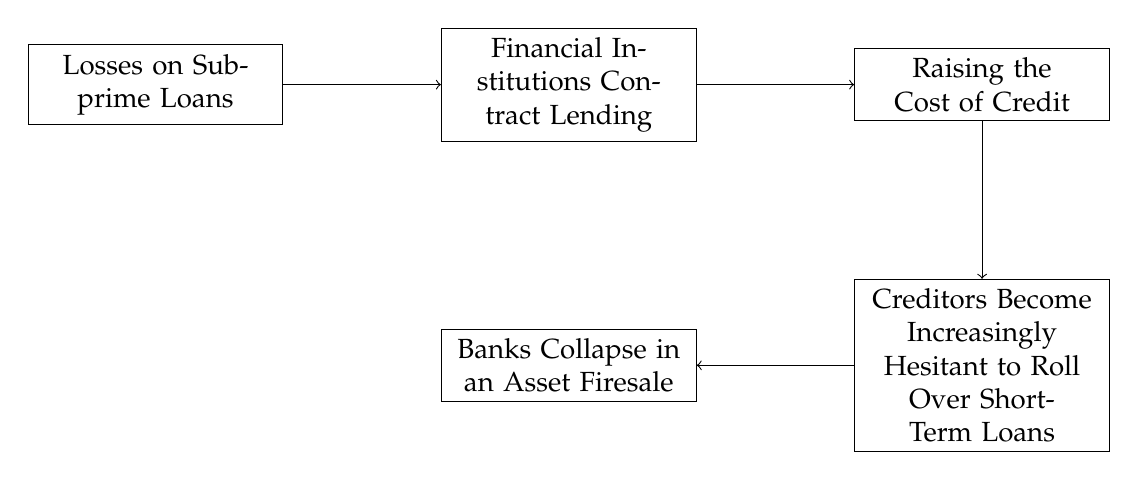
\begin{tikzpicture}[node distance=2cm]

        % Nodes
    \node (losses) [rectangle, draw, text width=3cm, text centered] {Losses on Subprime Loans};
    \node (financial) [rectangle, draw, text width=3cm, text centered, right=of losses] {Financial Institutions Contract Lending};
    \node (raising) [rectangle, draw, text width=3cm, text centered, right=of financial] {Raising the Cost of Credit};
    \node (creditors) [rectangle, draw, text width=3cm, text centered, below=of raising] {Creditors Become Increasingly Hesitant to Roll Over Short-Term Loans};
    \node (banks) [rectangle, draw, text width=3cm, text centered, left=of creditors] {Banks Collapse in an Asset Firesale};

        
        % Arrows
    \draw [->] (losses) -- (financial);
    \draw [->] (financial) -- (raising);
    \draw [->] (raising) -- (creditors);
    \draw [->] (creditors) -- (banks);
        
        \end{tikzpicture}
\end{frame}
%----------------------------------------------------------------------------------------
\begin{frame}{Relevant Literature}
    There are three key strands of literature present in this paper:
    \begin{itemize}
        \item Macroeconomic Models with a Banking Sector and Liqudity Risk (Gertler and Karadi (2011), Gertler and Kiyotaki (2011))
        \item Bank Runs (Diamond and Dybvig (1983), \textcolor{red}{Cole and Kehoe (2000)})
        \item Macroeconomic Models with Bank Runs (Ennis and Kiester (2003), Martin, Skeie, and von Thadden (2014))
    \end{itemize}
\end{frame}
%----------------------------------------------------------------------------------------
\begin{frame}{Relationship to BGG}
    Recall the notion of a financial accelerator in \textbf{Bernanke, Gertler and Gilchrist (1996)}:
    \begin{Definition}
        A financial accelerator is a mechanism by which shocks to the economy are propagated and amplified through credit markets
    \end{Definition}
    We will add to this financial accelerator by including a notion of bank runs, which further propagates economic shocks.
\end{frame}
%----------------------------------------------------------------------------------------
\section{Model}
%----------------------------------------------------------------------------------------
\begin{frame}{Environment}
    \begin{itemize}
        \item \textbf{Agents}: Households and Bankers, both of measure 1
        \item \textbf{Time}: Discrete, $t=0,1,2,...$
        \item \textbf{Goods}: A nondurable good and \textbf{capital}, a durable asset
        \begin{itemize}
            \item Capital does not depreciate and is fixed in total supply
            \item Capital is held by both banks and households, with $K_t^b+K_t^h=1$
        \end{itemize}
        \item \textbf{Shocks}: $Z_t$ is the shock to capital productivity, it is \textbf{aggregate}
    \end{itemize}
\end{frame}
%-----------------------------------------------------------------------------------------
\begin{frame}{Capital Evolution}
    The capital stock evolves differently depending on if it is held by \textbf{households} or \textbf{banks}:
    \begin{Definition}
        For banks, capital stock evolves as
        \begin{equation}
            K_{t}^b\rightarrow\begin{cases}
                Z_{t+1}K_t^b \text{ output }\\
                K_t^b \text{ capital }
            \end{cases}
        \end{equation}
    \end{Definition}
    \begin{Definition}
        For households, capital stock evolves as
        \begin{equation}
            \begin{cases}
                K_{t}^h \text{ capital }\\
                f(K_t^h) \text{ goods }
            \end{cases}
            \rightarrow\begin{cases}
                Z_{t+1}K_t^h \text{ output }\\
                K_t^h \text{ capital }
            \end{cases}
        \end{equation}
    \end{Definition}
\end{frame}
%-----------------------------------------------------------------------------------------
\begin{frame}{Why do bank runs occur?}
    Bank runs in this model are not classic bank runs, as in Diamond-Dybvig, but rather are generated
    by banks' inability to cover short term liabilities with long-term imperfectly liquid assets.
    \bigbreak 
    There are two key features of the model that lead to bank runs:
    \begin{itemize}
        \item Financing constraints on banks
        \item Inefficiencies in the home storage of capital
    \end{itemize}
    \bigskip
    We will be highlighting these more in the coming sections of the presentation, as households and 
    banks handle runs differently.
\end{frame}

%------------------------------------------------------------------------------------------
\section{Households}
%------------------------------------------------------------------------------------------
\begin{frame}{Households in Bank Runs}
    \begin{definition}
        \begin{equation}
        R_{t+1}
        \begin{cases}
            \Bar{R}_{t+1} \text{ if no bank run }\\
            x_{t+1} \Bar{R}_{t+1} \text{ if bank run }
        \end{cases}
    \end{equation}
    \end{definition}
\end{frame}
%------------------------------------------------------------------------------------------
\begin{frame}{Household Problem}
    \begin{Definition}
        The household problem can be expressed as the following: 
        \begin{multline}
                E_{t}\left[\sum^\infty_{i=0}\beta^i\ln(C_{t+i}^h)\right]\\
                \text{subject to } C_t^h+D_t+Q_t K_t^h + f(K_t^h) = Z_t W^h + \textcolor{red}{R_t D_{t-1}} + (Z_t +Q_t)K_{t-1}^h
        \end{multline}
    \end{Definition}
    \bigbreak
    \textbf{Importantly}, $R_t$ is the return on bank deposits in the \textbf{no run environment}, so we are assuming that 
    households do not anticipate bank runs. This assumption is relaxed in later sections.
\end{frame}
%-------------------------------------------------------------------------------------------
\begin{frame}{First Order Conditions for Households}
    \begin{itemize}
        \item Deposits (Household-Bank Interaction): $E_t(\Lambda_{t,t+1})R_{t+1}=1$ where $\Lambda_{t,t+1}=\beta^i\frac{C_t^h}{C_{t+i}^h}$
        \item Direct Capital Holdings of Households: $E_t(\Lambda_{t,t+1}R_{t+1}^h)=1$ with $R_{t+1}^h=\frac{Z_{t+1}+Q_{t+1}}{Q_t+f^\prime(K_t^h)}$
    \end{itemize}
    \bigbreak
    As $f^\prime(K_t^h)$ is increasing in capital held by the household, which means
    in the limiting case of a bank run, the price of capital drops sharply.
\end{frame}
%-------------------------------------------------------------------------------------------
\section{Banks}
%-------------------------------------------------------------------------------------------
\begin{frame}{Timing of Bank Decisions }
    \begin{figure}
        \centering
        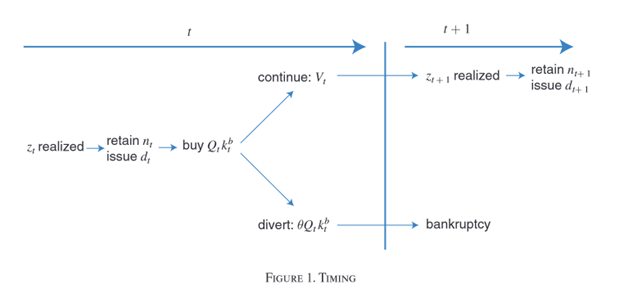
\includegraphics[scale=0.75]{banker_timing.png}
        \caption{Timing of Bank Decisions}
        \label{fig:my_label}
    \end{figure}
\end{frame}
%-------------------------------------------------------------------------------------------
\begin{frame}{Banker Problem}
    \begin{definition}
        The banker problem can be expressed as the following:
        \begin{multline}
            V_t=E_t\left[\sum^\infty_{i=1}\beta^i(1-\sigma)\sigma^{i-1}c_{t+i}^b\right]\\
        \end{multline}
        \begin{itemize}
            \item Bankers only consume in the last period of existence
            \item Bankers are risk neutral
            \item Bankers are finitely lived, dying with probability $1-\sigma$ each period (TV Condition)
        \end{itemize}
    \end{definition}
\end{frame}
%-------------------------------------------------------------------------------------------
\begin{frame}{Banker Net Worth Evolution}
    Bankers have evolving net worth based on their survival time:
    \begin{itemize}
        \item Bankers Born in Period $t$: $n_t=w^b$, net worth is equal to initial endowment
        \item Bankers Surviving from Period $t-1$: $n_t=(Z_t+Q_t)k^b_{t-1}-R_{t-1}D_{t-1}$, net worth is equal to return on capital from the previous period minus deposits
        \item Bankers Dying in Period $t$: $c_t^b=n_t$, bankers consume all their net wealth in the period they die
    \end{itemize}
    \begin{block}{Deposit Constraint}
        Bankers finance their asset holdings with deposits and equity, so $Q_tk_t^b=d_t+n_t$
    \end{block}
\end{frame}
%-------------------------------------------------------------------------------------------
\begin{frame}{Moral Hazard Problem}
    \begin{center}
        \textbf{Banks need a reason to limit the amount of issued deposits}
    \end{center}
    \bigbreak
    \begin{definition}
        Given the assumption that bankers can take $\theta Q_tk_t^b$ out of the bank without the investors knowing, we can
        write the \textbf{incentive constraint} for bankers as:
        \begin{equation}
            \theta Q_tk_t^b\leq V_t
        \end{equation}
        If this is not satisfied, households will not loan to firms as they have incentive to cheat.
    \end{definition}
\end{frame}

%-------------------------------------------------------------------------------------------
\begin{frame}{Restating the Banker Problem}
    Armed with all of this new information, we can restate the banker problem as:
    \begin{block}{Banker Problem}
        \begin{align*}
        &V_t=E_t\left[\beta(1-\sigma)n_{t+1}+\beta\sigma V_{t+1}\right]&\\
        &\text{subject to } \theta Q_tk_t^b\leq V_t&\\
        &\text{and } Q_tk_t^b=d_t+n_t&\\
        &\text{and } n_t=(Z_t+Q_t)k_{t-1}^b-R_{t}D_{t-1}&
    \end{align*}
    \end{block}
\end{frame}
%-------------------------------------------------------------------------------------------
\begin{frame}{Constraint Math}
    This is all extra math to generate a reframing of the Bank problem that we will see in the following slides.
    \begin{block}{Growth Rate of Net Worth}
        \begin{align*}
            \frac{n_{t+1}}{n_t}&=\frac{Z_{t+1}+Q_{t+1}}{Q_t}\frac{Q_tk^b_t}{n_t}-R_{t+1}\frac{d_t}{n_t}\\
            &=(R_{t+1}^b-R_{t+1})\phi_t+R_{t+1}
        \end{align*}
        subject to $R_{t+1}^b=\frac{Z_{t+1}+Q_{t+1}}{Q_t}$ and $\phi_t=\frac{Q_tk_t^b}{n_t}$
    \end{block}
$R_{t+1}^b$ can be thought of as the realized rate of return on bank assets, and $\phi$ is the ratio of assets to 
net worth.
\end{frame}
%-------------------------------------------------------------------------------------------
\begin{frame}{Tobin's Q Ratio}
    \begin{block}{Reframing of Tobin's Q}
        \begin{align*}
            \psi_t&=\underset{\phi_t}{\max}E_t\{\beta(1-\sigma+\sigma\psi_{t+1})\left[(R_{t+1}^b-R_{t+1})\phi_t+R_{t+1}\right]\}\\
            &=\underset{\phi_t}{\max}\{\mu_t\phi_t+\nu_t\}
        \end{align*}
        subject to the incentive constraint $\theta \phi_t \leq \psi_t=\mu_t\phi_t+\nu_t$ where $\mu_t=E_t\left[\beta\Omega_{t+1}(R_{t+1}^b-R_{t+1})\right]$ (excess marginal value of assets over deposits)
        and $\nu_t=E_t\left[\beta\Omega_{t+1}\right]R_{t+1}$ (marginal cost of deposits) with $\Omega_{t+1}\equiv 1-\sigma+\sigma\psi_{t+1}$ (discount factor weighting).
    \end{block}
\end{frame}
%-------------------------------------------------------------------------------------------
\begin{frame}{Relationship Between Incentive Constraint and $\mu_t$}
    Consider the following two environments, one where the incentive constraint exists and the other where it does not:
    \begin{itemize}
        \item \textbf{No Incentive Constraint}: Banks consume all excess return because they finance everything with deposits (infinite arbitrage),
        $R_{t}^b=R_t$ which then means $\mu_t=0$. \textbf{This is a frictionless, no run environment}.
        \item \textbf{Incentive Constraint}: This means that $\mu>0$, and banks will finance capital with their net worth after
        the incentive constraint binds, which is a textbook \textbf{financial accelerator}! If depositors choose not to roll
        over their deposits, this can be a bank run!
    \end{itemize}
\end{frame}
%-------------------------------------------------------------------------------------------
\begin{frame}{Aggregation (1)}
    \begin{block}{Assets and Net Worth}
        \begin{flalign*}
            Q_t K_t^b=\phi_t N_t
        \end{flalign*}
    \end{block}
    \begin{block}{Evolution of Net Worth}
        \begin{flalign*}
            N_t=\sigma\left[(Z_t+Q_t)K_{t-1}^b-R_tD_{t-1}\right]+W^B
        \end{flalign*}
    \end{block}
\end{frame}
%-------------------------------------------------------------------------------------------
\begin{frame}{Aggregation (2)}
    \begin{block}{Total Output}
        \begin{flalign*}
            Y_t=Z_t+Z_t W^h + W^b
        \end{flalign*}
    \end{block}
    \begin{block}{Economy Budget Constraint}
        \begin{flalign*}
            Y_t=f(K^h_t)+C_t^h+C_t^b
        \end{flalign*}
    \end{block}
\end{frame}
%-------------------------------------------------------------------------------------------
\section{Bank Runs}
%-------------------------------------------------------------------------------------------
\begin{frame}{Households are the problem!}
    Households choose not to roll over their deposits if:
    \begin{itemize}
        \item If they percieve other households will not do the same
        \item If the forced liquidation makes the banks insolvent
    \end{itemize}
\end{frame}
%-------------------------------------------------------------------------------------------
\begin{frame}{Condition for Runs to Exist}
    For runs to exist, we need to have the following condition:
    \begin{block}{Condition for Runs}
        \begin{flalign*}
            x_t=\frac{R_{t+1}^*}{R_{t+1}}=\frac{(Z_{t}+Q^*_{t})K^b_{t-1}}{R_{t}D_{t-1}}<1\\
            x_t=\frac{R_{t+1}^{b^*}}{R_{t+1}}\frac{\phi_{t-1}}{\phi_{t-1}-1}<1
        \end{flalign*}
    \end{block}
    with $R_{t+1}^{b^*}=\frac{Z_t+Q_t^*}{Q_{t-1}}$ and $\phi_t$ equal to the leverage mutliple,
    $\frac{Q_tK_t^b}{N_t}$.
\end{frame}
%-------------------------------------------------------------------------------------------
\begin{frame}{Run Threshold}
    \begin{figure}
        \centering
        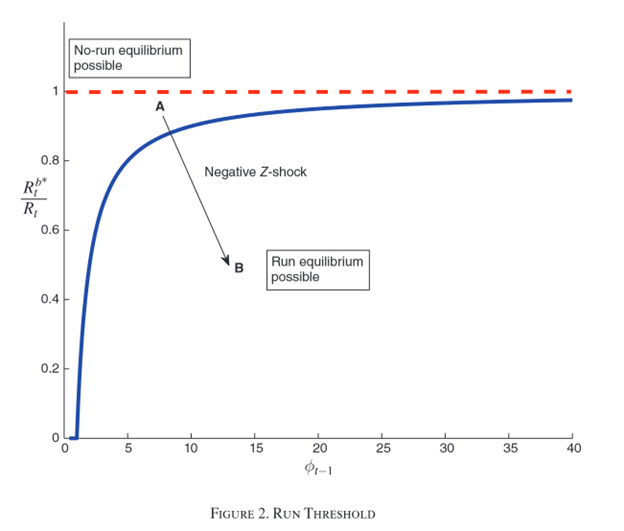
\includegraphics[scale=0.4]{run_threshold.png}
        \caption{Run Threshold}
        \label{fig:run_threshold}
    \end{figure}
\end{frame}
%-------------------------------------------------------------------------------------------
\begin{frame}{Bank Runs!}
    A bank run in $t$ works in the following way:
    \begin{enumerate}
        \item Households choose not to roll over their deposits en masse
        \item Banks are forced to liquidate assets to pay off depositors, moving \textbf{all} capital to the
        household sector, $K^H_t=1$
    \end{enumerate}
    \begin{block}{Banker Net Worth}
        \begin{flalign*}
            N_{t+1}&=W^b+\sigma(W^b)\\
            N_{t+j}&=W^b+\sigma((Z_{t+j}+Q_{t+j})K_{t+j-1}^b-R_{t+j}D_{t+j-1}) \text{ }\forall i\geq 2
        \end{flalign*}
    \end{block}
\end{frame}
%-------------------------------------------------------------------------------------------
\begin{frame}{Liquidation Price}
    Through some algebra, we can derive the liquidation price of capital for the household:
    \begin{block}{$Q^*$}
        \begin{flalign}
            Q^*_t=E_t\left[\sum^\infty_{i=0}\Lambda_{t,t+i}(Z_{t+i}-\alpha K^h_{t+i})\right]-\alpha
        \end{flalign}
    \end{block}
    \begin{itemize}
        \item $Z_t$ manifests in the equation, so $Q^{*}_t$ is vulnerable to fluctuations
        \item We notes that $Q^*_t$ is \textbf{decreasing} in $\alpha$
        \item $Q^*_t$ is \textbf{increasing} in $K_t^h$! The longer the banks remain insolvent,
        the lower the price of the fire sale of capital.
    \end{itemize}
\end{frame}
%-------------------------------------------------------------------------------------------
\begin{frame}{Liquidity Shortage and Insolvency}
    \textbf{If a bank run equilibrium exists}:
    \begin{itemize}
        \item Banks are insolvent when $Q_t=Q^*_t$
    \end{itemize}
    \textbf{If a bank run equilibrium does not exist}:
    \begin{itemize}
        \item Banks are solvent when $Q_t=Q_t$
    \end{itemize}
    \bigbreak
    \begin{centering}
        Asset price is based on liquidity which is effected by runs!
    \end{centering}
\end{frame}
%-------------------------------------------------------------------------------------------
\section{Impusle Response Functions}
%-------------------------------------------------------------------------------------------
\begin{frame}{Impulse Response Functions - No Runs}
    \begin{figure}
        \centering
        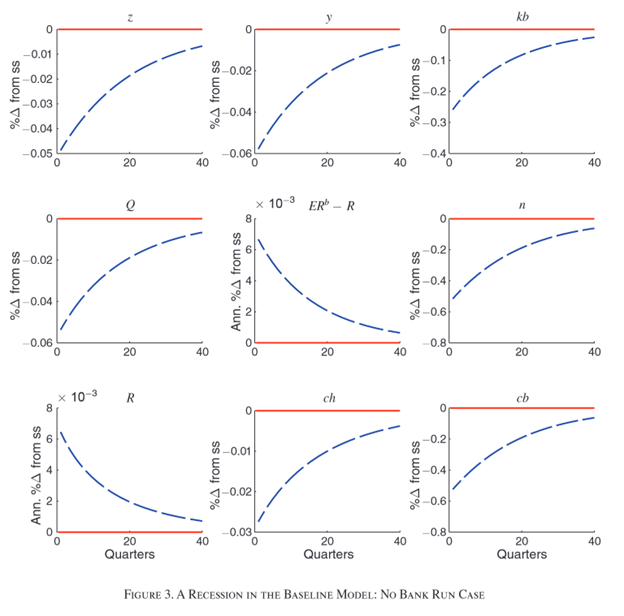
\includegraphics[scale=0.4]{no_run_case.png}
        \caption{Impulse Response Functions}
        \label{fig:irf}
    \end{figure}
\end{frame}
%-------------------------------------------------------------------------------------------
\begin{frame}{Impulse Response Functions - Runs}
    \begin{figure}
        \centering
        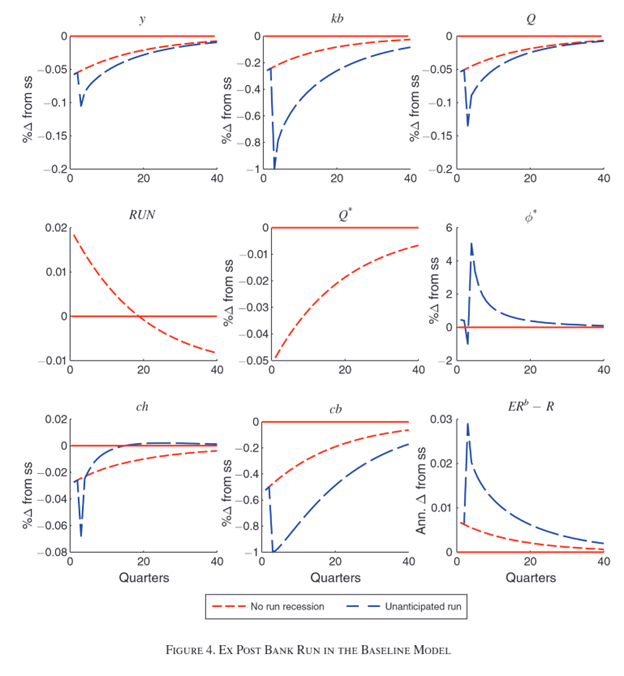
\includegraphics[scale=0.35]{run_case.png}
        \caption{Impulse Response Functions}
        \label{fig:irf_run}
    \end{figure}
\end{frame}
%-------------------------------------------------------------------------------------------
\begin{frame}{Anticipated Runs}
\begin{figure}
    \centering
    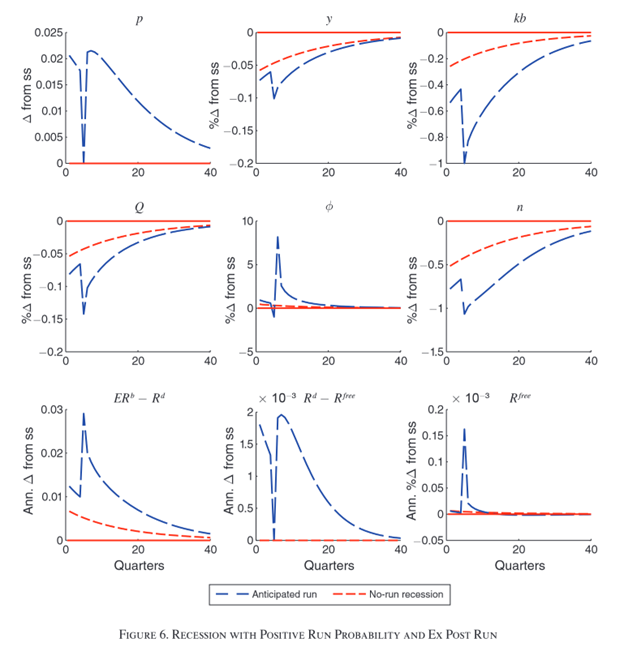
\includegraphics[scale=0.35]{run_case_expected.png}
    \caption{Impulse Response Functions}
    \label{fig:irf_anticipated}
\end{figure}
\end{frame}
%-------------------------------------------------------------------------------------------
\section{Conclusion}
%-------------------------------------------------------------------------------------------
\begin{frame}{What do we do?}
    The authors present problems, but they also present solutions:
    \begin{itemize}
        \item Deposit Insurance: Not possible  in the model due to violation of the incentive constraint
        \item \textbf{Capital Requirements}
        \item \textbf{Lender of Last Resort}
    \end{itemize}
\end{frame}
%-------------------------------------------------------------------------------------------
\begin{frame}{Conclusion}
    We have generated a model that has a traditional financial accelerator \textbf{and} liquidity mismatch leading to instability in the banking sector! 

    \bigbreak
    \begin{center}
        Questions?
    \end{center}
\end{frame}
\end{document}